\documentclass[10pt,a4paper, bibliography=totoc]{scrartcl}
\usepackage[utf8]{inputenc}
\usepackage[ngerman]{babel}
\usepackage{amsmath}
\usepackage{amsfonts}
\usepackage{amssymb}
\usepackage{marvosym}
%\usepackage{gensymb}
\usepackage{graphicx}
\usepackage{hyperref}
\usepackage{url}
\usepackage{float}
\usepackage{siunitx}
\usepackage{bookmark}
\usepackage{booktabs}
\sisetup{locale = DE}
\usepackage{subcaption}
\usepackage{listings}
\usepackage[settings]{markdown}
\usepackage{listingsutf8}
\usepackage{xcolor}

\definecolor{codegreen}{rgb}{0,0.6,0}
\definecolor{codegray}{rgb}{0.5,0.5,0.5}
\definecolor{codepurple}{rgb}{0.58,0,0.82}
\definecolor{backcolour}{rgb}{235, 235, 235}

\lstdefinestyle{mystyle}{
    backgroundcolor=\color{backcolour},   
    commentstyle=\color{codegreen},
    keywordstyle=\color{magenta},
    numberstyle=\tiny\color{codegray},
    stringstyle=\color{codepurple},
    basicstyle=\ttfamily\footnotesize,
    breakatwhitespace=false,         
    breaklines=true,                 
    captionpos=b,                    
    keepspaces=true,                 
    numbers=left,                    
    numbersep=5pt,                  
    showspaces=false,                
    showstringspaces=false,
    showtabs=false,                  
    tabsize=2
}
\lstset{style=mystyle, extendedchars=true, inputencoding=utf8}
\lstset{literate=%
  {Ö}{{\"O}}1
  {Ä}{{\"A}}1
  {Ü}{{\"U}}1
  {ß}{{\ss}}1
  {ü}{{\"u}}1
  {ä}{{\"a}}1
  {ö}{{\"o}}1
}
\usepackage[title,titletoc]{appendix}
\renewcommand{\appendixtocname}{Anhang}
\renewcommand{\appendixpagename}{Anhang}


%\renewcommand{\UrlFont}{\small\tt}
\usepackage[a4paper,lmargin={2.5cm},rmargin={2.5cm},tmargin={2.5cm},bmargin = {2.5cm}]{geometry}

\linespread{1.1}

\begin{document}

\pagenumbering{Roman}

\title{Radioastronomy}
\subtitle{Fortgeschrittenenpraktikum\\ HS1 Radioastronomy}
\author{Léonie Lanz \\ Nico Kalogerakis}
\maketitle
\newpage

\tableofcontents
\vfill
\newpage

\pagenumbering{arabic}

\section{Introduction}
The experiment HS1-Radioastronomy is there to give an overview for operating a radio telescope and to introduce the prerequitites such as characterising and calibrating the telescope before carrying out the experiments. The main experiment to be conducted is the observation of neutral hydrogen in the Milky Way to determine the rotational velocity in order to derive the mass distribution.

%Describe: aim of the practical experiment, procedure, the objective should be the rotation curve of the Milky Way in order to derive the mass distribution. Radio observations are particularly suitable for this purpose because, unlike optical observations, absorption by dust plays only a minor role. In addition, radio observations of the Earth’s surface are possible, which is otherwise only the case with optical observations. Here we can also briefly discuss the emission process behind the 21cm radiation
\section{Theoretical Background}

\subsection{Radioastronomy}

Radio astronomy is the study of electromagnetic radiation in the radio wavelength range, typically from a few MHz to several hundred GHz. Compared to optical astronomy, radio waves are much less affected by interstellar dust and gas, which allows astronomers to observe cold and dense regions of space that are often hidden in the optical regime. Radio telescopes usually consist of large parabolic antennas that collect incoming radiation and direct it to a receiver. The receiver amplifies the weak signal and converts it into an electrical voltage, from which the intensity, spectral distribution, and temperature of the observed source can be determined.

A central quantity in radio astronomy is the brightness temperature. In the Rayleigh-Jeans regime, which is valid for most radio astronomical observations, the spectral intensity is approximately
\[
I_\nu \approx \frac{2k_\mathrm{B} T_\mathrm{B} \nu^2}{c^2} = \frac{2k_\mathrm{B} T_\mathrm{B}}{\lambda^2},
\] 
% aus background 2.4.3 (gl 44)
where $I_\nu$ is the spectral intensity, $k_\mathrm{B}$ is the Boltzmann constant, $T_\mathrm{B}$ is the brightness temperature, $\nu$ is the frequency, and $c$ is the speed of light. This relation shows that the observed radio signal is directly linked to the temperature of the emitting medium. This makes radio astronomy a powerful method for studying cold molecular clouds, ionized gas regions, and neutral hydrogen structures in the Milky Way and beyond.

One of the most important spectral lines in radio astronomy is the 21 cm line emitted by neutral hydrogen.

\subsection{The 21 cm Hydrogen Line}

The hydrogen atom consists of a proton and an electron. In the ground state, the proton and electron spins can be oriented either parallel or antiparallel to each other. This gives rise to a hyperfine splitting of the ground state: the antiparallel configuration has a slightly lower energy than the parallel configuration. A transition from the higher-energy state to the lower-energy state leads to the emission of a photon with a frequency of approximately
\[
\nu \approx 1420.4\ \mathrm{MHz},
\]
which corresponds to a wavelength of
\[
\lambda \approx 21.1\ \mathrm{cm}.
\]
This transition is therefore called the 21 cm line.

This line is of great importance in astronomy because hydrogen is the most abundant element in the interstellar medium. Neutral hydrogen emits strongly at 21 cm, allowing astronomers to map the distribution of gas in galaxies. The 21 cm line is especially useful because it is only weakly absorbed by interstellar dust, so it can reveal regions that are difficult or impossible to observe in the optical range.

The 21 cm line also enables the measurement of Doppler shifts. If the hydrogen gas is moving relative to the observer, the frequency of the emission is shifted. From this shift, the radial velocity of the gas can be determined. This makes it possible to study galactic rotation, gas dynamics, and the mass distribution of galaxies. For this reason, the 21 cm line is one of the most important tools in modern radio astronomy and is fundamental for studying neutral hydrogen in the universe.


\section{Observation and Evaluation}
\subsection{The KRT3 telescope}

\subsection{Weather Conditions}
The experiment was carried out on 07.09.2026, starting at around 12:35. The weather was stable throughout the day with partial cloud coverage and temperatures around \qty{19}{\degree}.

\subsection{Calibration}
As the reciever recieves radiation not only from the source $T_S$ but also from the environment $T_h$. In addition to those two external sources of radiation, the antenna also picks up on the radiation it's own system emits $T_{sys}$. This means the measured power of the reciever, represented by the antenna temperature, can be broken down the following way:
\begin{align}
	T_A=T_S+T_h+T_{sys}
\end{align}
It is difficult to seperate the pure system temperature and the background radiation, so these temperatures are usually combined into an effective system temperature:
\begin{align}
	T'_{sys}=T_{sys}+T_h
\end{align}
The effective system temperature now includes all unwanted contributions. This means that to know the contribution of a source, one must know the effective system temperature. Determining the effective system temperature is calibrating the telescope by doing a 'On-Off' measurement through measuring a source with a known flux density and then measuring a piece of empty sky. The KRT3 however, can only measure the sun as a source with high enough flux density but the sun is not a constant source which is why a noise generator needs to be used.\\
The noise generator injects a signal directly into the antenna horn. The calibration temperature $T_{cal}=\qty{170}{K}$ is the expected antenna temperature that is observed additionally when the noise generator is switched on.\\
When assuming the sun to be a point-like source \autoref{eq:pointsrc} can be used in the form of:
\begin{align}
	T_b\Omega_s=T_A\Omega_A
\end{align}
with $T_b$ being the brightness temperature, $\Omega_s$ being the solid angle of the sun, $T_A$ being the antenna temperature and $\Omega_A$ being the solid angle of the antenna main lobe.\\
The goal is measuring the antenna temperature of the sun and converting it into a flux density. For this we need the following identities: the antenna theorem $A_e\Omega_A=\lambda^2$, the Rayleigh-Jeans law $B_\nu=2kT_b/\lambda^2$, the flux density $S_\nu=B_\nu\Omega_s$ and the aperture efficiency $\eta=A_e/A_g=0.5$ with $A_g$ being the geometric antenna surface assumed to be a circle.
\begin{align}
	T_b\Omega_s=T_A\Omega_A\\
	\Omega_{A}=\frac{\lambda^2}{A_{e}}, \Omega_{S}=\frac{S_{\nu}}{B_{\nu}}, B_{\nu}=\frac{2k_{B}T_{b}}{\lambda^2}\\
	S_{\nu}=\frac{T_{A}\cdot 2k_{B}}{A_{e}}=f(T_{A},A_{e})\\
	A_{e}=\pi r^{2}\cdot\eta=1,5^2\pi\cdot0,5=\pi\qty{1,125}{m^2}2\\
	\Rightarrow T_{A}=\frac{S_{\nu}A_{e}}{2k_{B}}=\frac{S_{\nu}\pi\qty{1,125}{m^2}}{2k_{B}}
\end{align}
\subsubsection{Determination of the system temperature}
\subsubsection{Background Radiation}
\subsection{Determination of the angular resolution of the KRT3}
The expected half-width is $q=1.02 \lambda /D= ...$ with the wavelength $\lambda=...$ and the antenna diameter $D=\qty{3}{m}$.

\subsection{Determination of the Sensitivity of the instrument}
To determine the theoretical sensitivity of the instrument, the weakest detectable flux density $\Delta S_\nu$ for a given system temperature $T'_{sys}$ can be given by the radiometer equation:
\begin{align}
\label{eq: radiometer}
\Delta S_\nu=\frac{2k}{A_e}\frac{C_sT'_{sys}}{\sqrt{\Delta\nu\tau}}
\end{align}
where $C_s\approx 2$ is a dimensionless instrumental constant and $\tau$ the integration time. 
With \autoref{eq: radiometer} the limiting sensitivity in a single channel with $\Delta\nu=\qty{61}{kHz}$ and an integration time of $\tau=\qty{1}{s}$ can be calculated to $\Delta S_\nu=...$.

The measurement is carried out with the radio source Vir A with an elevation of ...° at the time of measurement. The necessary integration time is calcuated to be $\tau=...$, taking the flux density at $\nu=\qty{1420.4}{MHz}$ to be $S_\nu=\qty{211}{Jy}\pm\qty{11}{Jy}$ after Baars et al. (1977). 

\subsection{Observation of neutral hydrogen in the Milky Way}
The preamplifier has a frequency range of 1398.00-1460.56 MHz divided into 1024 channels. The frequency resolution of a single channel (the bandwidth) is calculated ...
As we observe the H1 line in a single channel, the velocity resolution is ...
If we assume a radial velocity of 0 km/s 

\section{Results}

\subsubsection{Determination of the system temperature}
\subsubsection{Background Radiation}
\subsection{Determination of the angular resolution of the KRT3}
\subsection{Determination of the Sensitivity of the instrument}
\subsection{Observation of neutral hydrogen in the Milky Way}

%\begin{figure}[H]

    %\centering
    
    %\begin{subfigure}[b]{0.3\textwidth}
     %   \centering
     %   
\includegraphics[width=\linewidth]{img/strahltransport/02_schirm.png}
     %   \caption{Schirm 2}
     %   \label{fig:schirm2}
    %\end{subfigure}
    %\hfill
    %\begin{subfigure}[b]{0.3\textwidth}
     %   \centering
     %   
\includegraphics[width=\linewidth]{img/strahltransport/03_schirm.png}
     %   \caption{Schirm 3}
     %   \label{fig:schirm3}
    %\end{subfigure}

    %\caption{Gesamtdarstellung der fünf Messungen: Strahlprofile auf den verschiedenen Schirmen}
    %\label{fig:fuenf_bilder_gesamt}
%\end{figure}



\section{Discussion}


\section{Summary}


\newpage

\pagenumbering{Alph}

\bibliographystyle{ieeetr}
\bibliography{literatur}
%\addcontentsline{toc}{chapter}{Bibliography}

\newpage

\listoffigures 
\addcontentsline{toc}{section}{List of Figures}

\newpage

\appendix
\clearpage
\appendix
\clearpage
\addcontentsline{toc}{section}{Lab book}
%\section{Lab book}
\title{Labbook}
\date{07. - 09. September 2026}
\maketitle

\subsection*{Wetter}
\noindent
\textbf{Datum:} 07/09/26 \\
\textbf{Uhrzeit:} 12:35 Uhr \\

\begin{figure}[h]
     \centering
     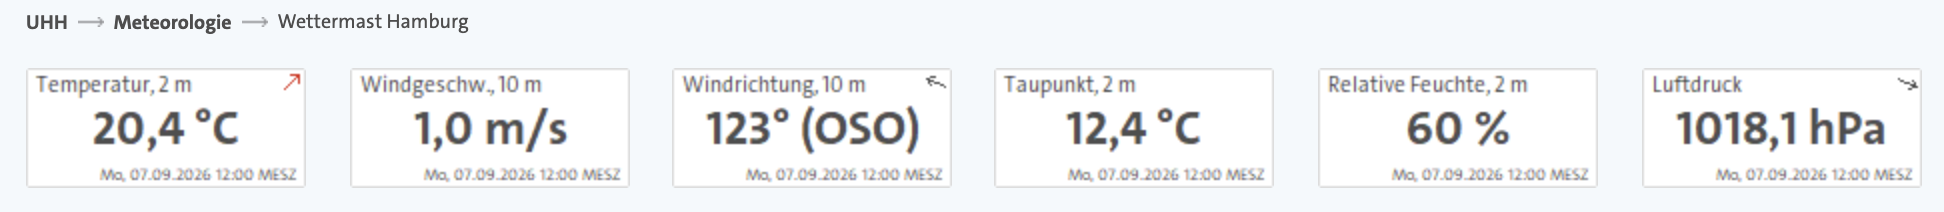
\includegraphics[scale=0.4]{img/labbook/wetter_hs1.png}
\end{figure}
\begin{itemize}
    \item Teilweise bedeckter Himmel
    \item Kein Niederschlag
\end{itemize}

\subsection*{5.1.1 Calibration (Systemtemperatur)}
USB 1-5, 9-13 \\
Datendatei-Struktur im Programm (RadioUniversePro):

\begin{table}[htbp]
\centering
\begin{tabular}{cccccccc}
\toprule
rep & dev & sb & on\_tbi & off\_tbi & cal\_tbi & flux & SEFD \\
\midrule
1 & bbc01 & u & 12195,30 & 1001,40 & 2634,20 & 00,00 & 00,00 \\
\bottomrule
\end{tabular}
\end{table}

\begin{align}
T_{b}\cdot \Omega_{S} &= T_{A}\Omega_{A} \\
\Omega_{A} &= \frac{\lambda^2}{A_{e}}, \quad \Omega_{S}=\frac{S_{\nu}}{B_{\nu}}, \quad B_{\nu}=\frac{2k_{B}T_{b}}{\lambda^2} \\
S_{\nu} &= \frac{T_{A}\cdot 2k_{B}}{A_{e}} = f(T_{A},A_{e}) \\
A_{e} &= \pi r^{2}\cdot\eta = 1,5^2\pi\cdot0,5 = 1,125\pi \, \text{m}^2 \\
T_{A} &= \frac{S_{\nu}A_{e}}{2k_{B}}
\end{align}

\begin{quote}
$T_{\text{sys,left}} = 98.76 \pm 22.54 \text{ K}$ \\
$T_{\text{sys,right}} = 107.80 \pm 31.65 \text{ K}$ \\
$T_{\text{sun,left}} = 1237.79 \pm 89.62 \text{ K}$ \\
$T_{\text{sun,right}} = 1302.59 \pm 119.16 \text{ K}$
\end{quote}

Mit $S_{\nu}$ der Sonne (aus SWC):
\begin{itemize}
    \item 76 sfu (solar flux units): $76 \cdot 10^{-11} \, \text{Wm}^{-2}\text{Hz}^{-1} = 76 \cdot 10000 \, \text{Jy} = 760000 \, \text{Jy}$
    \item $\Rightarrow T_A = 972,753 \text{ K}$
    \item Störung wegen RFI
\end{itemize}

\subsection*{5.2 Angular Resolution}
USB 1-5, 9-13 \\
Position der Sonne berechnet durch die Steuerungssoftware:

\begin{table}[htbp]
\centering
\begin{tabular}{cccccccc}
\toprule
Source & RA & DEC & AZ & EL & HA & Type & Note \\
\midrule
Sun & 110410.1 & +055810.9 & +1684733.7 & +42 00 48.8 & -003253.9 & Star & East \\
\bottomrule
\end{tabular}
\end{table}

\begin{itemize}
    \item Im Ordner \texttt{cscan} befindet sich der Screenshot.
    \item Im Ordner \texttt{FITS} befinden sich die Daten (lon vs. lat).
\end{itemize}

\subsection*{5.3 Sensitivity of the Instrument}
Antennentemperatur von VirA (BBC 3,11 zeigt geringsten RFI-Einfluss).

Benötigte Zeit für das Mapping:
\begin{itemize}
    \item 28:35.4s (Software)
    \item 29:27.8s (Eigener Timer)
\end{itemize}

\textit{Hinweis: Screenshot auf Ubuntu und nicht Windows! Files im Ordner \texttt{maps} und in \texttt{FITS} als \texttt{imageproJ01 VirA 01}.}

\subsubsection*{TODO: Theoretical Sensitivity}
\begin{align}
\Delta S_{\nu} &= \frac{2k}{A_{e}} \frac{C_{S}T'_{\text{sys}}}{\sqrt{\Delta \nu \tau}} \quad \text{(spektrale Flussdichte)}
\end{align}
Mit $C_{S} \approx 2$, $T'_{\text{sys,left}} = 98.76 \pm 22.54 \text{ K}$, $T'_{\text{sys,right}} = 107.80 \pm 31.65 \text{ K}$, $A_{e} = 1.125\pi$, $\tau = 1\text{s}$, $\Delta \nu = 61\text{kHz}$:
\begin{align}
\Delta S_{\nu,\text{left}} &= 6,248 \cdot 10^{-24} \frac{\text{W}}{\text{m}^2\text{Hz}} = 624,92 \text{ Jy} \\
\Delta S_{\nu,\text{right}} &= 6,82 \cdot 10^{-24} \frac{\text{W}}{\text{m}^2\text{Hz}} = 682,02 \text{ Jy}
\end{align}

Benötigte Integrationszeit $\tau$ zum Detektieren der ausgewählten Quelle mit dem KRT 3 mit einem Signal-Rausch-Verhältnis $S/N = 10$ in jedem Kanal:
\begin{itemize}
    \item Virgo A: Flussdichte $= 211 \pm 11 \text{ Jy}$, Radiogalaxie
    \item Für 5 Kanäle jede Seite ($\Delta \nu = 5 \cdot 61\text{kHz} = 305\text{kHz}$)
    \item $S/N = 10$
    \item Formel: $\tau = \left( \frac{2k\cdot C_{S}\cdot T'_{\text{sys}}}{\Delta S_{\nu}\cdot A_{E}} \right)^{2} \cdot \frac{\Delta\nu}{S/N}$
    \item $\tau_{l} = 4,12\text{s}$
    \item $\tau_{r} = 5,22\text{s}$
\end{itemize}

\subsubsection*{Determination of the Uncertainty of Radiant Flux Measurements}

\subsubsection*{Preliminary Work}
\begin{align}
S_{\nu} &= \frac{P}{4\pi d^2\sqrt{2\pi}\sigma} = 1263,16 \text{ Jy}
\end{align}
Für Mobile Radio on the Moon (übertragen mit 2W, 900MHz, FWHM: 80kHz, $\sigma = 34\text{kHz}$, empfangen auf der Erde).

\begin{align}
S_{\nu} &\propto \nu^{\alpha}, \quad \alpha = -0,7
\end{align}
Bei $\nu = 1420.4\text{ MHz}$: $S_{\nu,\text{CasA}} = 1420 \pm 70 \text{ Jy}$.
\begin{align}
c &= \frac{1420,4^{-0,7}\text{ MHz}}{1420\text{ Jy}} \\
S_{\nu,\text{Cas A}} &= \frac{900^{-0,7}}{c} \text{ Jy} = 1954,37 \text{ Jy} \\
T_{A} &= \frac{S_{\nu}A_{e}}{2k_{B}} = 1,82 \text{ K} \quad (\text{für } \nu = 1420.4\text{ MHz})
\end{align}

\noindent\textbf{TODO: Fehlerfortpflanzung}

\subsubsection*{Evaluation}
BBC 3,11
\begin{figure}[h]
     \centering
    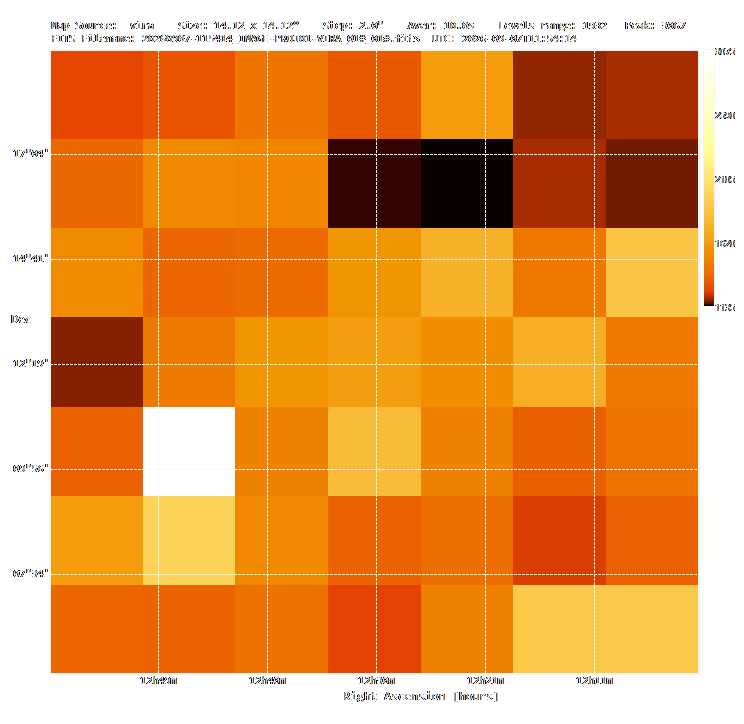
\includegraphics[scale=0.25]{img/labbook/map vira red.png}
\end{figure}
\begin{figure}[h]
     \centering
    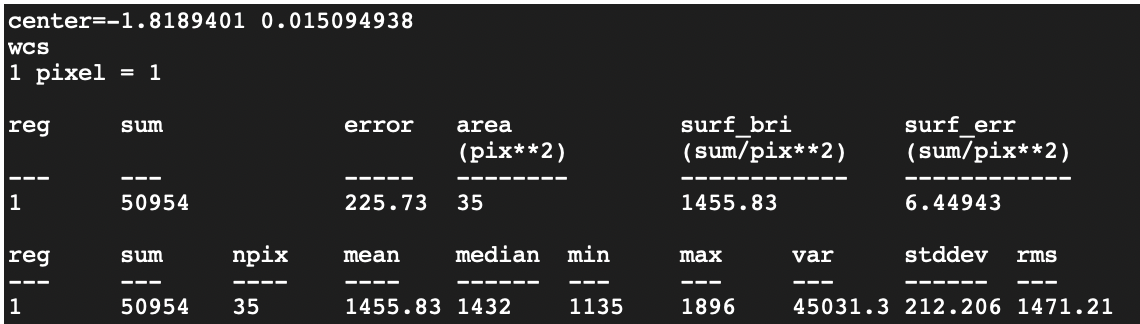
\includegraphics[scale=0.3]{img/labbook/ds9 region data.png}
\end{figure}
\begin{figure}[h]
     \centering
    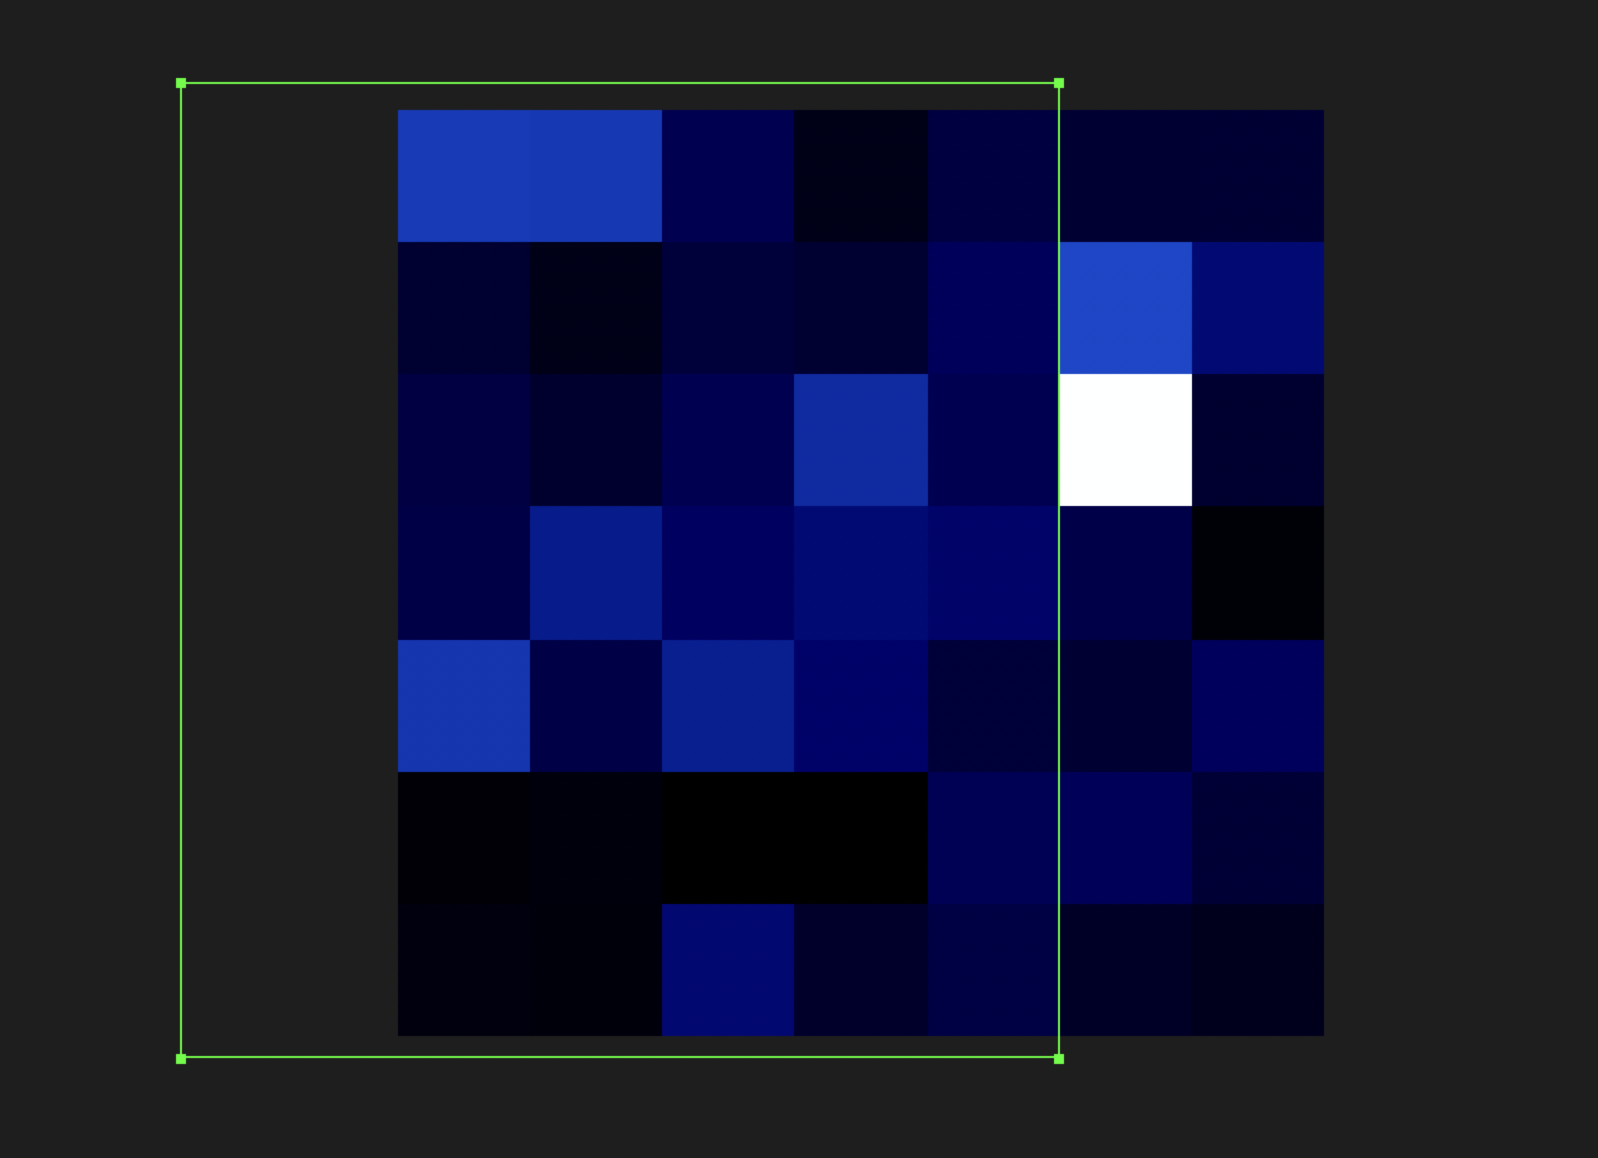
\includegraphics[scale=0.25]{img/labbook/ds9 region screenshot.png}
\end{figure}

\begin{align}
\text{mean} &= 1455,83 \\
\text{std} &= 212,206 \\
\sigma[K] &= \frac{\text{std}}{\text{mean}}\cdot T'_{\text{sys}} = 15,71 \text{ K} \\
\text{mean}_{\text{scaled}}[K] &= T_{A}(\text{OFF}) = 156938,474 \text{ K} \\
T_{A}(\text{ON}) &= 3067 \cdot 107,8\text{K} = 330622,6 \text{ K}
\end{align}

Antennentemperatur der Quelle:
\begin{align}
T_{s} &= \frac{T_{A}(\text{ON})-T_{A}(\text{OFF})+T'_{\text{sys}}}{T'_{\text{sys}}} = 1612,17 \text{ K}
\end{align}

\begin{itemize}
    \item Rauschen ist viel größer als erwartet.
    \item Vergleich mit theoretischer Empfindlichkeit (600 Jy, ca. 1 K).
    \item Bei uns jetzt 128 Kanäle, 10s Integrationszeit $\rightarrow$ eigentlich sollte es noch besser sein ($\ll 1\text{ K}$).
    \item Bei uns jedoch viel Einfluss von RFI $\rightarrow \sim 15\text{ K}$ Std./Rauschen.
    \item Empfänger-/Verstärkersensibilität ist ein Problem; thermisches Rauschen begrenzt nicht, aber besser als 1 K kann es eigentlich nicht werden.
\end{itemize}

Gesucht: $S/N$ (25 Karten für $S/N = 10$).

\subsection*{5.1.2 Background Radiation}
\subsubsection*{Mond}
Elevation: $30^\circ \, 52' \, 32.0''$ (in Grad, Minuten, Sekunden) \\
Für BBC 1-5, 9-13 (wie zuvor für die Sonne, auch bei schlechter Qualität).
\begin{align}
\text{Span} &= 2(\text{ELV} - 10^\circ) = 2(30^\circ - 10^\circ) = 40^\circ
\end{align}
Da der Azimut bei $268^\circ \, 03' \, 32.7''$ liegt, wählen wir einen etwas kleineren Span: $\text{Span} = 38^\circ$. \\
Zeitpunkt: ca. 14:56 Uhr. \\
Daten in FITS: \texttt{LON-MOON} und \texttt{LAT-MOON} + Screenshot in \texttt{cscan}: \texttt{CSCAN-MOON}.

\subsubsection*{Virgo A}
Zeitpunkt: 15:28 Uhr \\
Elevation: $47^\circ \, 56' \, 18''$, Azimut: $196^\circ$, $\text{Span} = 74$.

\subsection*{Observation of Neutral Hydrogen in the Milky Way}
\subsubsection*{Frequency Setting of the Receiver}
\subsubsection*{Preliminary Work}
\begin{itemize}
    \item Was ist die Frequenzauflösung $\delta\nu$ (Bandbreite eines einzelnen Kanals) und wie lautet die Geschwindigkeitsauflösung $\delta\upsilon$ bei der Beobachtung der H I-Linie?
    \item In welchem Kanal würden Sie die H I-Linie bei $\nu_0 = 1420.4\text{ MHz}$ erwarten, unter Annahme einer Radialgeschwindigkeit von $0\text{ km s}^{-1}$?
    \item Sie wollen das Radiokontinuum einer Quelle messen. Welche Frequenzen sind innerhalb der Bandbreite erlaubt, damit die Messung nicht durch die 21cm-Linie kontaminiert wird? (Maximale Radialgeschwindigkeit des H I: $\pm 200\text{ km s}^{-1}$).
    \item Welche Frequenzbänder sollten in BBC Tools ausgewählt werden, wenn man einmal die H I-Linie und einmal das Kontinuum beobachten möchte?
\end{itemize}

\subsubsection*{Measurement}
\begin{align}
R &= R_{0}\cdot \sin(l), \quad R_{0} = 8,5\text{ kpc}
\end{align}

\begin{table}[htbp]
\centering
\begin{tabular}{cccc}
\toprule
$l$ [deg] & $R$ [kpc] & $v_{\max}$ [km/s] & $v_{R}$ [km/s] \\
\midrule
10 & $1,48 \pm 4,09$ & -- & -- \\
20 & $2,91 \pm 4,0$ & $70,70 \pm 14,50$ & $\dots$ \\
\bottomrule
\end{tabular}
\end{table}

\begin{itemize}
    \item $v_{\max}$ grafisch bestimmt (Schnittwert mit der orangen $\sigma$-Linie).
    \item $v_{R} = v_{\max} + \omega_{0}R_{0}\cdot \sin(l)$ mit $\omega_{0}R_{0} = 220\text{ km/s}$.
    \item $v_{\max,\text{err}}$ grafisch über blauen Bereich bestimmt (Schnittpunkt min -- Schnittpunkt max / 2).
    \item $\Delta l = \pm 2^\circ$.
    \item Fehlerfortpflanzung für $R$:
    \begin{align}
    \Delta R &= \left|\frac{\partial R}{\partial l}\right|\cdot \Delta l = |R_{0}\cdot \cos(l)|\cdot \Delta l \\
    \sigma_{R} &= \sqrt{|R_{0}\cos(l)|\Delta l}
    \end{align}
    \item Eingeschlossene Masse:
    \begin{align}
    M(R) &= 0,234 \cdot 10^{10} \left( \frac{v(R)}{100\text{ km/s}} \right)^2 \left( \frac{R}{\text{kpc}} \right) M_{\odot}, \quad 1 M_{\odot} = 1,98 \cdot 10^{30}\text{ kg}
    \end{align}
\end{itemize}

\subsubsection*{Distribution of Dark Matter}
\begin{align}
M_{\text{DM}}(R_0) &= 66411575447.22 \pm 3593349279.00 \, M_{\odot}
\end{align}

\end{document} 